
\section{Introdução}


\noindent \begin{minipage}[c]{0.6\textwidth}
  \vspace {1cm}
  \par Esta presente aula prática tem por fim a aplicação dos paradigmas da linguagem orientada a objetos com a linguagem de programação Java\ref{fig:log_java}.
  \par Para os procedimentos práticos foi sugerido o uso de nome $gerenciaBanco$, o qual será implementado. A finalidade desta aula prática, visa a implementação de um sistema de gerenciamento de banco, aonde o cliente deste banco irá acendero sistema atravéz de uma interface gráfica através da biblioteca $java.swing.*$, o menu deverá ser do tipo $loop$ o usuário deverá escolher a oção de finalizar a operação.

\end{minipage}
\begin{minipage}[c]{0.4\textwidth}

  
\includegraphics[width=\textwidth]{figure/log_java.jpg}
  	\label{fig:log_java}
    \captionof{figure}{Logo Java, \citeonline{logJava}}
    %\captionof*{figure}{Fonte: \citeonline{linux:2023}}
\end{minipage}

\par As funções para este programa são:
\begin{itemize}
  \item Incerção das credenciais (Nome, Sobrenome e cpf);
  \item Consulta de saldo;
  \item Depósito;
  \item Saque;
  \item Finaliza a operação com uma mensagem de despedida;
\end{itemize}

\par Segundo \citeonline{freecodecamp:2023}, a linguagem orientata a objetos se define em quatro pilares, sendo elas: herança, encapsulamento, abstração e poliformismo. Isso permite definir, neste caso, umas características de \textbf{cliente}, e utiliza-lós inúmeras vezes sem a necessidade de rescreve-lá.

\section{Métodos}
\par Para a confecção desta aula prática, foi criado um \href{https://github.com/OgliariNatan/gerenciaBanco}{repositório no \textbf{Github}}, com o objetivo do aplicar os controle de versões e a utilização do sistema \textit{git} em geral, o relatório foi confeccionado em \LaTeX\, com o objetivo da abstração da formatação do texto ficando livre para o aprofundamento na questão textual.


\par De forma subsequente as instruções do \href{https://github.com/OgliariNatan/gerenciaBanco/blob/main/Aula%20pr%C3%A1tica.pdf}{roteiro da aula prática} é criado um projeto no NetBeans em java conforme figura \ref{fig:project}.

\begin{figure}[h!]
  \centering
  \subfigure[Início projeto.\label{fig:pro1}]{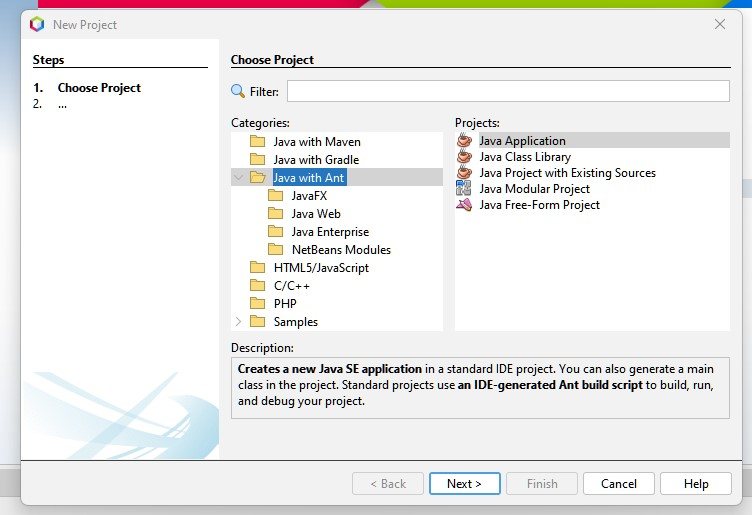
\includegraphics[scale=.4]{figure/fig_1.jpg}}
  \subfigure[Nome projeto.\label{fig:pro2}]{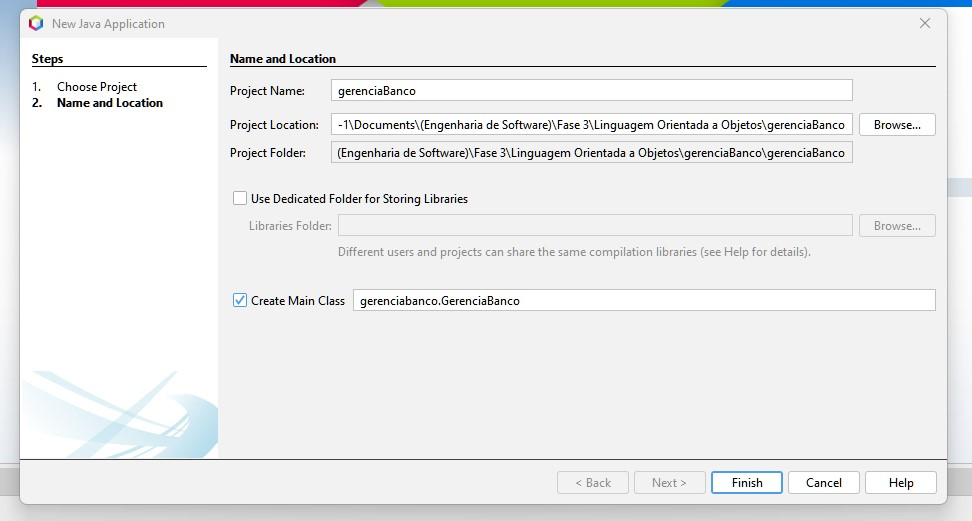
\includegraphics[scale=.4]{figure/fig_2.jpg}}
  \subfigure[Projeto em branco.\label{fig:pro3}]{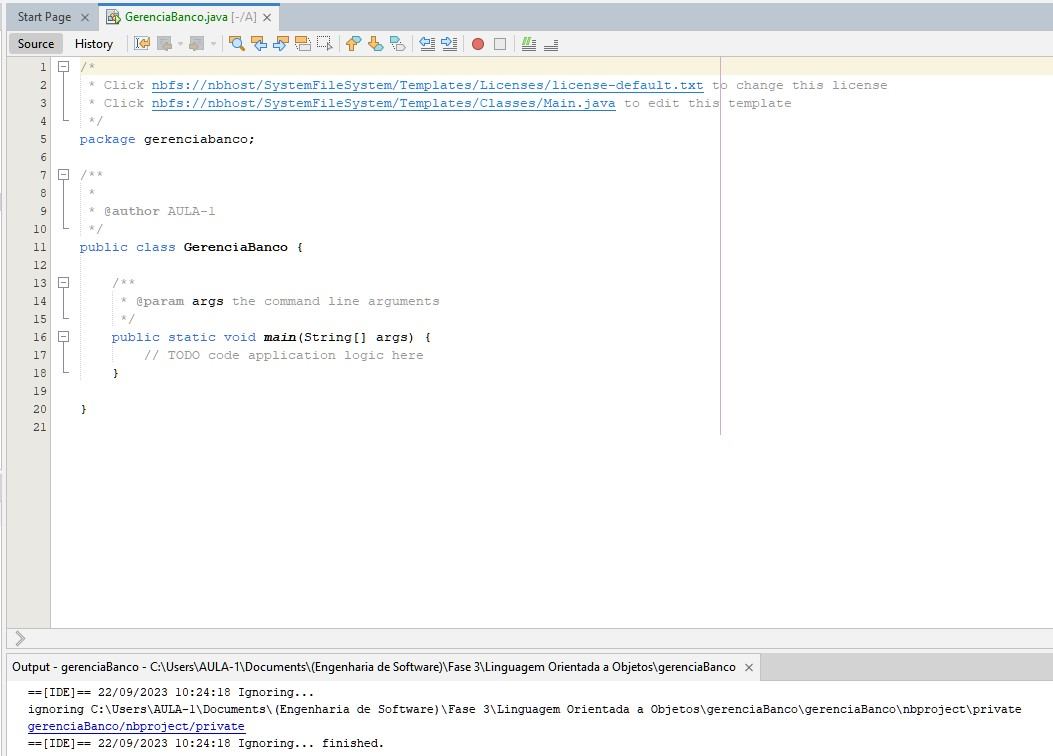
\includegraphics[scale=.4]{figure/fig_3.jpg}}
  \caption{Projeto java, O autor (2023)}\label{fig:project}
\end{figure}

\newpage

\par Na figura \ref{fig:pro1} solicita o tipo de projeto a ser criado, no caso \textit{Java Application}, na figura \ref{fig:pro2} é solicitado o local aonde o projeto será salvo e o nome do mesmo, deste modo o nome foi definido conforme sugestão do roteiro \textit{gerenciaBanco} e na figura \ref{fig:pro3} demonstra a criação do projeto em \textbf{branco} já com a inclusão do pacote \textit{gerenciabanco},após  estes passos foi prossegido com a programação do que foi solicitado ao discente.

\par Para organização desta aula prática foi confeccionado um diagrama UML para o programa, conforme demonstra a figura \ref{fig:uml}

\begin{figure}[h!]
  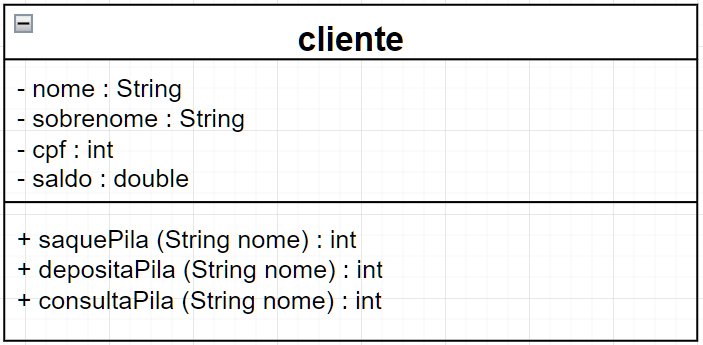
\includegraphics[width=\textwidth]{figure/uml_classe.png}
  \caption{Diagrama UML, O autor (2023)}
  \label{fig:uml}
\end{figure}

\newpage

\par Forãm definidos atributos para a classe e o mesmos são:
\begin{itemize}
  \item name : String
  \item sobrenome : String
  \item cpf : String
  \item saldo : double
\end{itemize}

\par Seguindo boas práticas de programação, define-se variáveis de controle de erros, e para tal, a criação de constatnte de verificação em vez de zeros e uns (0,1), do tipo $private static final int  STATUS\_OK = 1;$ e $private static final int STATUS\_FAIL = 0;$.


\section{Resultados}

\par Após a criação dos repositórios e do projeto, prossegue com a confecção do código\footnote{\hyperref[anexo]{código completo}}, no decorrer desta seção será incluido figuras dos resultados da presente aula.




\subsection{Métodos das classes}

\par Os métodos definem as ações da classe, e o acesso é $minhaClasse.meuMetodo(args)$

\begin{lstlisting}[language=Java, caption=consultaPilas, label=consultaPilas]
    /**
    * Realiza a consulta do saldo de uma conta
    * @param nome Passa o nome da conta a ser consultada e informa o saldo ao cliente.
    */
     public double consultaPilas(String nome){
     JOptionPane.showMessageDialog(null,"Seu saldo atual e de: R$" +this.saldo, this.nome+" "+this.sobrenome, JOptionPane.INFORMATION_MESSAGE, icon);
     }
\end{lstlisting}



\begin{lstlisting}[language=Java, caption=depositoPilas, label=depositaPilas]
  /**
   * Realiza um depósito em uma conta
   * @param nome Informa o nome da conta a ser depositado
   * @return retorna STATUS_OK se a operacao ocorreu com sucesso e retorna STATUS_FAIL se ocorrer um erro
   */
   public void depositaPila( String nome){
          try {// verifica se a entrada e do tipo numeral
              double pilaDeposito = Double.parseDouble(JOptionPane.showInputDialog(null,"Informe a quantidade em Reais (R$) a ser depositado na conta do "+this.nome+" "+this.sobrenome));
                this.saldo += pilaDeposito;
               //JOptionPane.showMessageDialog(null,"Seu Saldo e R$:"+this.consultaPilas(this.nome)+" Reais", this.nome, JOptionPane.INFORMATION_MESSAGE, icon);
               return STATUS_OK;
           }

           catch (NumberFormatException e) {// imprime o erro na tela e informa o que foi digitado.
               JOptionPane.showMessageDialog(null,"Entre com valor valido, do tipo numeral.\n Use (.) ponto em vez de (,) virgula\n ERRO: " + e.getMessage()  , "ERRO", JOptionPane.ERROR_MESSAGE);
               return STATUS_FAIL;
           }
   }
\end{lstlisting}




\section{Conclusões}

\par Esta aula prática teve como fim a aplicação de conhecimentos adquiridos em sala de aula virtuais da disciplina de linguagem orientada a objetos do curso bacharel em engenharia de software da faculdade UNOPAR,

o código completo\footnote{\hyperref[anexo]{código completo}}  pode ser visto nos anexos\ref{anexo} deste documento.

  %$X \xLongleftarrow[\text{NATAN}]{\text{OGLIARI}} Y $ %COM TEXTO
	% $\uparrow$ %Seta para Cima
	%$\overleftarrow{NATAN}$
